\documentclass[
  11pt,
  letterpaper,
   addpoints,
   answers
  ]{exam}

\usepackage{../exercise-preamble}

\begin{document}

\noindent
\begin{minipage}{0.47\textwidth}

\includegraphics[width=\textwidth]{../fcfm_die}
\end{minipage}
\begin{minipage}{0.53\textwidth}
\begin{center} 
\large\textbf{Electromagnetismo Aplicado} (EL3103-1) \\
\large\textbf{Clase auxiliar extra} \\
\normalsize Prof.~Benjamin Jacard H.\\
\normalsize Prof.~Aux.~Erik Saez A.
\end{center}
\end{minipage}

\vspace{0.5cm}
\noindent
\vspace{.85cm}
\begin{questions}
    %%%%%%%%%%%%%%%%%%%%%%%%%%%%
    \question Resuelva los siguientes problemas basados en el esquema de la figura
    \begin{itemize}
    \item[(a)] Las expresiones para el campo eléctrico $\mathcal{E}$ y la intensidad magnética $\mathcal{H}$.
    
    \item[(b)] Obtenga una expresión para $E_1^{-}$ (onda reflejada del medio 1), tal que esta dependa de $(E_2^{-}, Y_2, Y_3, Y_1)$ considerando una distancia $d = \frac{\lambda}{4}$.
    
    \item[(c)] Sea el caso en que $\varepsilon_2 = \sqrt{\varepsilon_1 \varepsilon_3}$, demuestre en base a la expresión anterior que no existirá onda reflejada en el medio 1. \textit{Hint}: ocupar la siguiente expresión:
    \begin{align}
    (b + c)(b - a) + (b + a)(b - c) = (b^2 - ac) \tag{1}
    \end{align}
\end{itemize}
  \begin{center}
        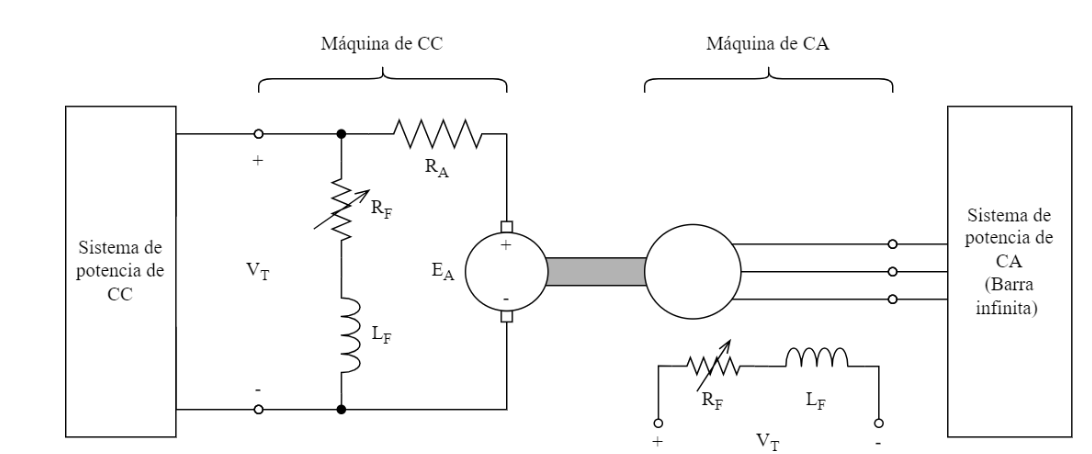
\includegraphics[width=0.5\textwidth]{Auxiliar_6_1}
        \captionof{figure}{Esquema de los dielectricos}
      \end{center}
    %%%%%%%%%%%%%%%%%%%%%%%%%%%
    \begin{solution}
        \begin{itemize}
            \item Se tiene las siguientes expresiones para los campo es eléctricos y magnéticos según los medios y las zonas de interés:
\subsection*{\underline{Campo eléctrico e intensidad magnética z $\leq$ d}}
\begin{align}
    E_{1}&= E_{1}^{+}e^{-j\beta z} + E_{1}^{-}e^{j\beta z}\\
    H_{1}&= Y_{1}E_{1}^{+}e^{-j\beta z} - Y_{1}E_{1}^{-}e^{j\beta z}
\end{align}
\subsection*{\underline{Campo eléctrico e intensidad magnética eléctricos d $\leq$ z $\leq$ 0}}
\begin{align}
    E_{2}&= E_{2}^{+}e^{-j\beta z} + E_{2}^{-}e^{j\beta z}\\
    H_{2}&= Y_{2}E_{2}^{+}e^{-j\beta z} - Y_{2}E_{2}^{-}e^{j\beta z}
\end{align}
\subsection*{\underline{Campo eléctrico e intensidad magnética eléctricos z $\geq$ 0}}
\begin{align}
    E_{3}&= E_{3}^{+}e^{-j\beta z} + 0\\
    H_{3}&= Y_{3}E_{3}^{+}e^{-j\beta z} + 0
\end{align}
Teniendo la consideración que en el medio 3 no habrá onda reflejada si no que solo transmitida
\item Se busca el obtener una relación para la intensidad de campo eléctrico $E_{1}^{-}$ tal que dependa de las variables ($E_{2}^{-}, Y_{2} , Y_{3} , Y_{1}$), con lo que se evaluaran en las diferentes interfaces tal que permitan utilizar condiciones de borde.
\subsection*{\underline{Primera condición}}
\begin{align}
    E_{1}(z=-d) &= E_{2}(z=-d)\\
    E_{1}^{+}e^{j\beta d} +E_{1}^{-}e^{-j\beta d} &= E_{2}^{+}e^{j\beta d} +E_{2}^{-}e^{-j\beta d}
\end{align}
Luego se evaluando en d=$\lambda/4$ se tendrá:
\begin{align}
    E_{1}^{+}(j)+ E_{1}^{-}(-j) &= E_{2}^{+}(j)+ E_{2}^{-}(-j)\\
    E_{1}^{+} -E_{1}^{-} &= E_{2}^{+}- E_{2}^{-}
\end{align}
De manera análoga para la intensidad de campo magnético:
\begin{align}
    H_{1}(z=-d) &= H_{2}(z=-d)\\
    Y_{1}E_{1}^{+}e^{j\beta d} -Y_{1}E_{1}^{-}e^{-j\beta d} &= Y_{2}E_{2}^{+}e^{j\beta d} -Y_{2}E_{2}^{-}e^{-j\beta d}\\
    Y_{1}E_{1}^{+}(j) - Y_{1}E_{1}^{-}(-j) &= Y_{2}E_{2}^{+}(j) - Y_{2}E_{2}^{-}(-j)\\
    Y_{1}E_{1}^{+} + Y_{1}E_{1}^{-} &= Y_{2}E_{2}^{+}+ Y_{2}E_{2}^{-}
\end{align}
\subsection*{\underline{Segunda condición}}
\begin{align}
    E_{2}(z=0) &= E_{3}(z=0)\\
    E_{2}^{+}e^{j\beta \cdot 0} +E_{2}^{-}e^{-j\beta \cdot 0} &= E_{3}^{+}e^{j\beta \cdot 0}\\
    E_{2}^{+} + E_{2}^{-} &= E_{3}^{+}
\end{align}
\begin{align}
    H_{2}(z=0) &= H_{3}(z=0)\\
    Y_{2}E_{2}^{+}e^{j\beta \cdot 0} - Y_{2}E_{2}^{-}e^{-j\beta \cdot 0} &= Y_{3} E_{3}^{+}e^{j\beta \cdot 0}\\
    Y_{2}E_{2}^{+} - Y_{2}E_{2}^{-} &= Y_{3}E_{3}^{+}
\end{align}
Luego se obtienen las ecuaciones que nos permitirán obtener lo buscando , tal que:
\begin{align}
    Y_{2}E_{2}^{+} - Y_{2}E_{2}^{-} &= Y_{3}E_{3}^{+}\\
    Y_{2}E_{2}^{+} - Y_{2}E_{2}^{-} &= Y_{3}(E_{2}^{+}+E_{2}^{-})\\
    Y_{2}E_{2}^{+} - Y_{2}E_{2}^{-} &= Y_{3}E_{2}^{+}+ Y_{3}E_{2}^{-}\\
    E_{2}^{+}(Y_{2} - Y_{3}) &= E_{2}^{-}(Y_{2}+Y_{3})\\
    E_{2}^{+} &= E_{2}^{-}\frac{(Y_{2} + Y_{3})}{(Y_{2}-Y_{3})} 
\end{align}
Se tendrá por otro lado que:
\begin{align}
    E_{1}^{+} -E_{1}^{-} &= E_{2}^{+}- E_{2}^{-}\\
                      E_{1}^{+}   &= E_{2}^{+}- E_{2}^{-}+ E_{1}^{-}\\ 
\end{align}
Luego reemplazando esta expresión en lo siguiente:
\begin{align}
    Y_{1}E_{1}^{+} + Y_{1}E_{1}^{-} &= Y_{2}E_{2}^{+}+ Y_{2}E_{2}^{-}\\
    Y_{1}(E_{2}^{+}- E_{2}^{-}+ E_{1}^{-})+ Y_{1}E_{1}^{-} &= Y_{2}E_{2}^{+}+ Y_{2}E_{2}^{-}\\
    Y_{1}E_{2}^{+} - Y_{1}E_{2}^{-} + 2Y_{1}E_{1}^{-} &= Y_{2}E_{2}^{+} + Y_{2}E_{2}^{-}\\
\end{align}
Dado que se busca el obtener explícitamente la expresión $E_{1}^{-}$ , despejando en base a lo anterior se tendrá:
\begin{align}
      E_{1}^{-} &= \frac{E_{2}^{+}(Y_{2}-Y_{1}) + E_{2}^{-}(Y_{2}+Y_{1})}{2Y_{1}}\\
\end{align}
Considerando la ecuación de borde obtenida con anterioridad:
\begin{align}
    E_{2}^{+}= \frac{E_{2}^{-}(Y_{2}+Y_{3})}{(Y_{2}-Y_{3})}
\end{align}
Por tanto
\begin{align}
      E_{1}^{-} &=  \frac{E_{2}^{-} \left( \frac{(Y_{2}+Y_{3})(Y_{2}-Y_{1})}{(Y_{2}-Y_{3})}+(Y_{2} + Y_{1}) \right)}{2Y_{1}}
\end{align}
Finalmente se obtiene una expresión para $E_{1}^{-}$ en términos de las variables buscadas.
\item Se busca el analizar la situación en que $\epsilon_{2}= \sqrt{\epsilon_{1} \cdot \epsilon_{3}}$ , por lo volviendo sobre la ecuación anterior.
\begin{align}
      E_{1}^{-} &=  \frac{E_{2}^{-} \left( \frac{(Y_{2}+Y_{3})(Y_{2}-Y_{1})}{(Y_{2}-Y_{3})}+(Y_{2} + Y_{1}) \right)}{2Y_{1}}\\
      &= \frac{ E_{2}^{-}( (Y_{2}+ Y_{3}) (Y_{2}-Y_{1}) + (Y_{2}+Y_{1})(Y_{2}-Y_{3}))}{2Y_{1}(Y_{2}-Y_{3})}
\end{align}
Utilizando lo siguiente:
\begin{align}
    (b+c)(b-a)+ (b+a)(b-c) = (b^{2} - ac)
\end{align}
Con lo que la expresión se reduce:
\begin{align}
    E_{1}^{-} = \frac{E_{2}^{-}(Y_{2}^{2} - Y_{1}Y_{3})}{2Y_{1}(Y_{2}-Y_{3})}
\end{align}
Luego tomando el numerador de la expresión anterior y recordando que la admitancia viene dada por $Y= \sqrt{\frac{\epsilon}{\mu}}$
\begin{align}
    Y_{2}^{2} - Y_{1}Y_{3}&= \left( \sqrt{\frac{\epsilon_{2}}{\mu_{0}}} \right)^{2} - \left(\sqrt{\frac{\epsilon_{1} \cdot \epsilon_{3}}{\mu_{0}^{2}}}\right)\\
    &= \frac{\epsilon_{2}}{\mu_{0}} - \frac{\sqrt{\epsilon_{1}\cdot\epsilon_{3}}}{\mu_{0}}\\
    &= \frac{\sqrt{\epsilon_{1}\cdot\epsilon_{3}}}{\mu_{0}} - \frac{\sqrt{\epsilon_{1}\cdot\epsilon_{3}}}{\mu_{0}}\\
    &=0
\end{align}
Con lo que bajo la condición inicial se obtiene que $E_{1}^{-}= 0$, es decir que no se tendrá onda reflejada en el medio 1.
        \end{itemize}
    \end{solution}
    %%%%%%%%%%%%%%%%%%%%%%%%%%%%
    \question 
    Considere una onda plana cuyo campo eléctrico tiene magnitud $E_0$ y dirección $\hat{x}$, incidiendo normalmente en una placa dieléctrica imperfecta de permitividad $\varepsilon = \varepsilon' - j \varepsilon''$ y espesor $d$.

    \begin{enumerate}
        \item[(a)] Los campos totales $E(z)$ y $H(z)$ en todas las regiones.
        \item[(b)] El coeficiente de reflexión $\Gamma(z)$ en $z = -d$.
        \item[(c)] La potencia disipada en el dieléctrico y la potencia de la onda transmitida en el medio 3, considerando unidad de área en el plano $xy$.
\end{enumerate}
   
\textbf{Datos:}
\begin{itemize}
    \item $|E_0| = 1~[\mathrm{V/m}]$ (valor máximo)
    \item $f = 10~\mathrm{GHz}$
    \item $d = 1~\mathrm{cm}$
    \item $\varepsilon_r' = 2.5$, \quad $\varepsilon_r'' = 0.1$
\end{itemize}
    \begin{center}
        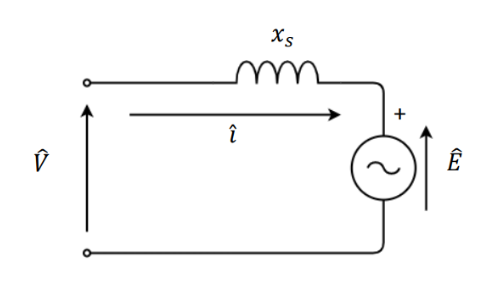
\includegraphics[width=0.5\textwidth]{Auxiliar_6_2}
        \captionof{figure}{Esquema de los dielectricos}
      \end{center}
    %%%%%%%%%%%%%%%%%%%%%%%%%%%%
    \begin{solution}
         \begin{enumerate}
            \item Dado que se trabajan en diferentes medios, se debe considerar la permitividad y permeabilidad de cada medio. En este caso, se tiene:
\begin{align*}
\text{Medio 1:} & \quad \varepsilon_0,\ \mu_0 \\
\text{Medio 2:} & \quad \varepsilon_2 = \varepsilon = \varepsilon' - j \varepsilon'' = (\varepsilon_r' - j \varepsilon_r'') \varepsilon_0 \\
\text{Medio 3:} & \quad \varepsilon_3 = \varepsilon_0 \\
& \quad k_0 = \omega \sqrt{\mu_0 \varepsilon_0} = \frac{2\pi}{\lambda_0}, \quad \lambda_0 = \frac{c}{f}, \quad c = 3 \times 10^8 \,\text{[m/s]} \\
& \quad Y_0 = \sqrt{\frac{\varepsilon_0}{\mu_0}}
\end{align*}
Luego tenemos que los campos electricos y magnéticos en cada medio seran los siguientes:
\textbf{Medio 1:}
\begin{align*}
\vec{E}_1 &= \left( E_0 e^{-j k_0 z} + E_r e^{j k_0 z} \right) e^{j \omega t} \, \hat{x} \\
\vec{H}_1 &= \left( Y_0 \, \hat{k} \times E_0 e^{-j k_0 z} \hat{x} + Y_0 (-\hat{k}) \times E_r e^{j k_0 z} \hat{x} \right) e^{j \omega t} \\
&= \left( Y_0 E_0 e^{-j k_0 z} \hat{y} + Y_0 E_r e^{j k_0 z} (-\hat{y}) \right) e^{j \omega t}
\end{align*}

% Medio 2
\textbf{Medio 2:}
\begin{align*}
\vec{E}_2 &= \left( E_2^+ e^{-j k_2 z} + E_2^- e^{j k_2 z} \right) e^{j \omega t} \, \hat{x} \\
\vec{H}_2 &= Y_2 \left( E_2^+ e^{-j k_2 z} \hat{y} + E_2^- e^{j k_2 z} (-\hat{y}) \right) e^{j \omega t} 
\end{align*}
Luego tenemos las siguientes relaciones dadas por:
\begin{align*}
k_2 &= \omega \sqrt{\mu_0 \varepsilon_2} = \beta_2 - j \alpha_2 \quad \text{donde } j k_2 = \alpha + j \beta \\
Y_2 &= Y_0 \sqrt{\varepsilon_{2r}} = \sqrt{\frac{\varepsilon_2}{\mu_0}} \\
\varepsilon_{2r} &= \frac{\varepsilon_2}{\varepsilon_0}
\end{align*}

\textbf{Medio 3:}
\begin{align*}
\vec{E}_3 &= E_3^+ e^{-j k_3 z} \hat{x} \, e^{j \omega t} \\
\vec{H}_3 &= Y_3 \, \hat{k} \times \vec{E}_3 = Y_3 E_3^+ e^{-j k_3 z} \hat{y} \, e^{j \omega t} \\
k_3 &= k_0, \quad Y_3 = Y_0
\end{align*}

\item Se busca obtener el coeficiente de reflexión \( \Gamma \) en la interfaz \( z = -d \). Recordando que este coeficiente nos indica la relación entre la onda reflejada y la onda incidente, se tiene:
\begin{equation}
\Gamma = \frac{E_1^- e^{-j k_0 d}}{E_0 e^{j k_0 d}} = \frac{E_1^-}{E_0} e^{-j 2 k_0 d}
\end{equation}
Para determinar \( E_1^- \), se deben imponer condiciones de frontera para los campos \( \vec{E} \) y \( \vec{H} \) en las interfaces \( z = 0 \) y \( z = -d \):

\paragraph{En \( z = 0 \):}
\begin{align}
E_2 &= E_3 \Rightarrow E_2^+ + E_2^- = E_3^+ \\
H_2 &= H_3 \Rightarrow Y_2 (E_2^+ - E_2^-) = Y_3 E_3^+
\end{align}

\paragraph{En \( z = -d \):}
\begin{align}
E_1 &= E_2 \Rightarrow E_0 e^{j k_0 d} + E_1^- e^{-j k_0 d} = E_2^+ e^{j k_2 d} + E_2^- e^{-j k_2 d} \\
H_1 &= H_2 \Rightarrow Y_0 (E_0 e^{j k_0 d} - E_1^- e^{-j k_0 d}) = Y_2 (E_2^+ e^{j k_2 d} - E_2^- e^{-j k_2 d})
\end{align}
De las relaciones entre \( E_2^+ \) y \( E_2^- \) para z=0, tenemos que:
\begin{align}
Y_2 \left( \frac{E_2^+ - E_2^-}{E_2^+ + E_2^-} \right) = Y_3
\Rightarrow Y_2 E_2^+ - Y_2 E_2^- = Y_3 E_2^+ + Y_3 E_2^- \\
(Y_2 - Y_3) E_2^+ = (Y_2 + Y_3) E_2^-
\end{align}
Luego las expresiones para \( \Gamma \) son las siguientes:
\begin{align}
1 + \Gamma &= \frac{E_2^+ e^{j k_2 d} + E_2^- e^{-j k_2 d}}{E_0 e^{j k_0 d}} \\
1 - \Gamma &= \frac{Y_2}{Y_0} \cdot \frac{E_2^+ e^{j k_2 d} - E_2^- e^{-j k_2 d}}{E_0 e^{j k_0 d}}
\end{align}
Luego tenemos que:
\begin{align}
\frac{1 - \Gamma}{1 + \Gamma} &= \frac{Y_2}{Y_0} \cdot \frac{E_2^+ e^{j k_2 d} - E_2^- e^{-j k_2 d}}{E_2^+ e^{j k_2 d} + E_2^- e^{-j k_2 d}}
\end{align}

Sustituyendo \( E_2^- = \frac{Y_2 - Y_3}{Y_2 + Y_3} E_2^+ \), obtenemos:
\begin{align}
\frac{1 - \Gamma}{1 + \Gamma} &= \frac{Y_2}{Y_0} \cdot \frac{(Y_2 + Y_3)e^{j k_2 d} - (Y_2 - Y_3)e^{-j k_2 d}}{(Y_2 + Y_3)e^{j k_2 d} + (Y_2 - Y_3)e^{-j k_2 d}}
\end{align}

\begin{equation}
\Gamma = \frac{1 - \dfrac{Y_2}{Y_0} \cdot \dfrac{(Y_2 + Y_3)e^{j k_2 d} - (Y_2 - Y_3)e^{-j k_2 d}}{(Y_2 + Y_3)e^{j k_2 d} + (Y_2 - Y_3)e^{-j k_2 d}}}
{1 + \dfrac{Y_2}{Y_0} \cdot \dfrac{(Y_2 + Y_3)e^{j k_2 d} - (Y_2 - Y_3)e^{-j k_2 d}}{(Y_2 + Y_3)e^{j k_2 d} + (Y_2 - Y_3)e^{-j k_2 d}}}
\end{equation}

De la condición en \( z = -d \) tenemos:
\begin{align}
E_0 e^{j k_0 d} + E_1^- e^{-j k_0 d} &= E_0 e^{j k_0 d}(1 + \Gamma) = E_2^+ e^{j k_2 d} + E_2^- e^{-j k_2 d} \\
\frac{Y_0}{Y_2} (E_0 e^{j k_0 d} - E_1^- e^{-j k_0 d}) &= \frac{Y_0}{Y_2} E_0 e^{j k_0 d} (1 - \Gamma) = E_2^+ e^{j k_2 d} - E_2^- e^{-j k_2 d}
\end{align}

Sumando y restando:
\begin{align}
E_0 e^{j k_0 d}(1 + \Gamma) + \frac{Y_0}{Y_2} E_0 e^{j k_0 d}(1 - \Gamma) &= 2 E_2^+ e^{j k_2 d} \\
E_0 e^{j k_0 d}(1 + \Gamma) - \frac{Y_0}{Y_2} E_0 e^{j k_0 d}(1 - \Gamma) &= 2 E_2^- e^{-j k_2 d}
\end{align}

Finalmente,de las ecuaciones anteriores se determina:
\begin{equation}
E_3^+ = E_2^+ + E_2^-
\end{equation}
     \item La potencia que se transmite al medio \( 3 \) se determina con el vector de Poynting y queda dada por:
\begin{align}
P_{\text{trans}}^{\text{medio 3}} &= \frac{1}{2} \Re\left\{ \vec{E}_3^+ \times \vec{H}_3^{+*} \cdot \hat{k} \right\} \\
&= \frac{1}{2} Y_3 \left| E_3^+ \right|^2
\end{align}

La potencia que entra a la placa dieléctrica está dada por la diferencia entre la potencia de la onda incidente y la potencia de la onda reflejada en la interfaz \( z = -d \):
\begin{align}
P_{\text{trans}}^{\text{placa diel.}} &= P_{\text{inc}} - P_{\text{refl}} \bigg|_{z = -d} \\
&= P_{\text{inc}} (1 - \rho^2), \quad \text{en que } \rho = |\Gamma| \\
&= \frac{1}{2} Y_0 |E_0|^2 (1 - \rho^2)
\end{align}

La potencia disipada en la placa dieléctrica queda dada por:
\begin{equation}
P_{\text{disip}}^{\text{placa diel.}} = P_{\text{trans}}^{\text{placa diel.}} - P_{\text{trans}}^{\text{medio 3}}
\end{equation}

La constante de propagación en el medio \( 2 \) está dada por:
\begin{align}
j k_2 &= j \omega \sqrt{\mu_0 \varepsilon_2} = j \omega \sqrt{\mu_0 (\varepsilon_2' - j \varepsilon_2'')} = \alpha_2 + j \beta_2
\end{align}

\begin{align}
\alpha_2 &= \omega \sqrt{\frac{\mu_0 \varepsilon_2'}{2} \left( \sqrt{1 + \left( \frac{\varepsilon_2''}{\varepsilon_2'} \right)^2} - 1 \right)} \\
\beta_2 &= \omega \sqrt{\frac{\mu_0 \varepsilon_2'}{2} \left( \sqrt{1 + \left( \frac{\varepsilon_2''}{\varepsilon_2'} \right)^2} + 1 \right)}
\end{align}

Luego el factor de propagación

\begin{align}
e^{j k_2 d} &= e^{\alpha_2 d + j \beta_2 d} = e^{\alpha_2 d} e^{j \beta_2 d} = e^{\alpha_2 d} (\cos \beta_2 d + j \sin \beta_2 d) \\
e^{-j k_2 d} &= e^{-\alpha_2 d - j \beta_2 d} = e^{-\alpha_2 d} (\cos \beta_2 d - j \sin \beta_2 d)
\end{align}


Para los cálculos numéricos es necesario trabajar con unidades del sistema MKS:

\begin{align*}
|E_0| &= 1\ \left[\frac{\text{V}}{\text{m}}\right], & f &= 10^{10}\ [\text{Hz}], & \omega &= 2 \pi f \\
d &= 0{,}01\ [\text{m}], & \varepsilon_0 &= \frac{1}{36\pi} \times 10^{-9}\ \left[\frac{\text{F}}{\text{m}}\right] \\
\varepsilon_2' &= 2{,}5\, \varepsilon_0, & \varepsilon_2'' &= 0{,}1\, \varepsilon_0 \\
\mu_0 &= 4\pi \times 10^{-7}\ \left[\frac{\text{H}}{\text{m}}\right]
\end{align*}

         \end{enumerate}
    \end{solution}
     
    
%%%%%%%%%%%%%%%%%%%%%%%%%%%
\end{questions}
\newpage
%%%%%%%%%%%%%%%%%%%%%%%%%%%

\end{document}